\documentclass{article}
\usepackage[utf8]{inputenc}
\usepackage[T1]{fontenc}
\usepackage[italian]{babel}
\usepackage{hyperref}
\usepackage{amsmath}
\usepackage{graphicx,subcaption,lipsum} %per migliore flessibilità con grafici
\usepackage{diagbox}
\usepackage{amsfonts}
\usepackage{mathtools}
\usepackage{subfiles}
\usepackage{caption}

\renewcommand{\labelitemi}{-}

\def \-> {\rightarrow}


\usepackage{booktabs}
\usepackage{siunitx}

\usepackage{geometry}
\usepackage{hyperref}
\usepackage[document]{ragged2e}
 \geometry{
 a4paper,
 total={170mm,257mm},
 left=20mm,
 top=20mm,
 }

\title{\textbf{Colorazione di grafi con Graph Neural Networks\\
e minimizzazione differenziabile dell'energia di Potts}}
\author{Gruppo 6: Mauro Bellucci, Marta Pizzo, Marco Tornambè}
\date{Corso di Metodi AI per la Fisica - ML 2026}

\begin{document}

\maketitle

\begin{abstract}
In questo lavoro viene presentato un metodo basato su Graph Neural Networks (GNN) per
affrontare il problema della colorazione di grafi tramite ottimizzazione differenziabile.
La GNN assegna a ciascun nodo una distribuzione di probabilità sui colori disponibili e
viene addestrata minimizzando un'energia di Potts differenziabile, arricchita da un termine
entropico con peso decrescente, utilizzando l'ottimizzatore Adam di PyTorch. La colorazione
discreta finale si ottiene con un argmax sull'output della rete. Il metodo è stato applicato
a due grafi in formato DIMACS: \texttt{g11} (25 nodi, 160 archi) e \texttt{g17} (128
nodi, 2113 archi). Per \texttt{g11} è stata trovata una colorazione valida con $c = 5$
colori in 5 esecuzioni su 50, stabilendo $\chi(\texttt{g11}) \leq 5$. Per \texttt{g17}
è stata trovata una colorazione valida con $c = 35$ colori in 1 esecuzione su 50,
stabilendo $\chi(\texttt{g17}) \leq 36$.
\end{abstract}

\section{Introduzione al problema}

Il problema della \textbf{colorazione di grafi} è così definito: dato un grafo non orientato $G = (V, E)$,
dove $V$ è l'insieme dei nodi e $E$ quello degli archi, si vuole assegnare a ciascun nodo
$i \in V$ un colore scelto da un insieme finito di $c$ colori, in modo tale che nessuna
coppia di nodi adiacenti condivida lo stesso colore:
\begin{equation}
    \forall\,(i,j) \in E: \quad \mathrm{color}(i) \neq \mathrm{color}(j).
\end{equation}

Il \textbf{numero cromatico} $\chi(G)$ è il minimo intero $c$ per cui esiste una
colorazione valida di $G$. Determinare esattamente $\chi(G)$ è un problema NP-completo
per grafi generali: non è noto alcun algoritmo polinomiale esatto, e i metodi di ricerca
esaustiva diventano proibitivi già per grafi di medie dimensioni.

In questo progetto viene adottato un approccio basato su reti neurali:
anziché cercare la soluzione con un algoritmo combinatorio esatto, si formula il problema
come \emph{ottimizzazione differenziabile} e lo si risolve con una GNN addestrata
direttamente sul grafo di interesse.

I due grafi assegnati al Gruppo 6 sono stati scaricati dal repository del corso in formato
DIMACS standard:
\begin{itemize}
    \item \texttt{g11}: 25 nodi, 160 archi non orientati.
    \item \texttt{g17}: 128 nodi, 2113 archi non orientati.
    \end{itemize}
    Rappresentazioni grafiche dei due grafi sono riportati in Figura \ref{fig:grafiNoColor}

 \begin{figure}[htb!]
  \centering
  \begin{subfigure}{0.45 \textwidth}
    \centering
    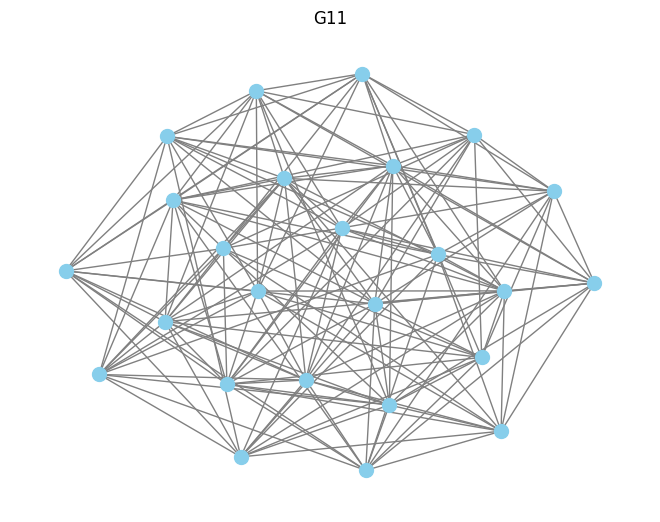
\includegraphics[width = 1 \textwidth]{g11NoColor}
    \caption{Rappresentazione di g11.}
    \label{fig:g11NoColor}
  \end{subfigure}
  \hfill
  \begin{subfigure}{0.45 \textwidth}
    \centering
    \includegraphics[width = 1 \textwidth]{g17NoColor}
    \caption{Rappresentazione di g17.}
    \label{fig:g17NoColor}
  \end{subfigure}
    \caption{Rappresentazione grafica dei grafi.}
  \label{fig:grafiNoColor}

\end{figure}

Come confronto iniziale, l'algoritmo greedy \texttt{greedy\_color} di NetworkX (strategia
\textit{largest\_first}, che ordina i nodi per grado decrescente) ha prodotto una
colorazione con $c = 7$ colori per \texttt{g11} e $c = 32$ colori per \texttt{g17}.
Questi valori costituiscono limiti superiori di riferimento per $\chi(G)$.

\section{Strategia Utilizzata}

%\subsection*{Riformulazione come ottimizzazione differenziabile}

L'idea centrale del metodo è quella di trasformare il problema discreto di
colorazione in un problema continuo. Invece di assegnare direttamente un colore intero a
ogni nodo, la GNN produce per ciascun nodo $i$ un vettore di probabilità sui $c$ colori
disponibili (ottenuti tramite softmax dell'output della rete):

\begin{equation}
    p_i = \bigl(p_{i1},\, p_{i2},\, \dots,\, p_{ic}\bigr), \qquad
    \sum_{k=1}^c p_{ik} = 1, \quad p_{ik} \geq 0.
\end{equation}
Il valore $p_{ik}$ rappresenta la probabilità assegnata al colore $k$
per il nodo $i$. 
L'addestramento minimizza una funzione di perdita differenziabile che
penalizza le assegnazioni in conflitto. Al termine, la colorazione discreta si ottiene
tramite argmax.

%\subsection*{Funzione di loss: energia di Potts differenziabile}
La funzione di perdita è ispirata all'\textbf{hamiltoniana antiferromagnetica del modello
di Potts}. Nel modello di Potts antiferromagnetico su reticolo, l'energia è minima quando
spin adiacenti si trovano in stati diversi. Pre ottenere una funzione differenziabile sui vettori di probabilità, si definisce:
\begin{equation}
    \mathcal{L}_{\mathrm{Potts}} = \sum_{(i,j)\in E} p_i \cdot p_j
    = \sum_{(i,j)\in E} \sum_{k=1}^c p_{ik}\, p_{jk}.
\end{equation}
Ogni termine $p_i \cdot p_j$ misura la \emph{sovrapposizione} tra le distribuzioni di
colore dei due nodi estremi dell'arco $(i,j)$. Se i nodi tendono ad assumere lo stesso
colore, il prodotto scalare è grande (fino a 1 nel caso di vettori one-hot identici) e
contribuisce ad aumentare la loss. Se i nodi tendono a colori diversi, il prodotto è
piccolo e la loss è ridotta. Minimizzare $\mathcal{L}_{\mathrm{Potts}}$ spinge quindi la
rete a produrre assegnazioni in cui nodi adiacenti hanno colori diversi.

%\subsection*{Regolarizzazione con termine entropico}


Per velocizzare l'addestramento (favorendo assegnazioni più nette) è stato aggiunto alla loss un termine entropico:
\begin{equation}
    H = -\frac{1}{|V|} \sum_{i \in V} \sum_{k=1}^c p_{ik} \log p_{ik},
\end{equation}
in modo che la loss totale sia:
\begin{equation}
    \mathcal{L}_{\mathrm{tot}} = \mathcal{L}_{\mathrm{Potts}} + \lambda\, H.
\end{equation}
All'inizio dell'allenamento il peso entropico è nullo, per permettere alla rete di esplorare in libertà la loss-landscape, il valore viene poi aumentato nel corso dell'addestramento.

Al termine dell'addestramento, la colorazione discreta è ottenuta assegnando a ogni nodo
il colore con probabilità massima:
\begin{equation}
    \mathrm{color}(i) = \arg\max_k\, p_{ik}.
\end{equation}
Il numero di \textbf{conflitti residui} $N_{\mathrm{conflicts}}$ è il numero di archi
$(i,j)$ per cui $\mathrm{color}(i) = \mathrm{color}(j)$. Una colorazione è valida se e
solo se $N_{\mathrm{conflicts}} = 0$.

Per stimare $\chi(G)$, l'intero processo (costruzione della rete, addestramento,
discretizzazione) viene ripetuto per valori crescenti di $c$, con più inizializzazioni
casuali indipendenti per ogni $c$. Il numero cromatico stimato è il minimo $c$ per cui
almeno un'esecuzione produce $N_{\mathrm{conflicts}} = 0$.

\section{Architettura della rete}

La rete utilizzata è denominata \texttt{ColoraGrafo} ed è implementata in PyTorch con la
libreria \texttt{PyTorch Geometric}. L'architettura è composta da quattro blocchi
principali.

\begin{itemize}
\item [-] \textbf{Embedding iniziale dei nodi}: A ciascun nodo $i$ è associato un vettore di embedding appreso tramite uno strato
\texttt{nn.Embedding}: ogni nodo viene identificato dal proprio indice intero e mappato in
$\mathbb{R}^h$, dove $h$ è la dimensione nascosta. Questo approccio consente alla rete di
apprendere una rappresentazione specifica per ogni nodo del grafo di input, non condizionata
da feature esterne. Poiché il metodo addestra una GNN separata per ciascun grafo, questa
scelta è coerente con l'obiettivo: ottimizzare i parametri per il singolo grafo assegnato.
\item [-] \textbf{Layer di message passing: SAGEConv}: L'embedding di ciascun nodo viene aggiornato attraverso 2 strati di convoluzione \textbf{SAGEConv}, separati da attivazioni
ReLU. 
\item [-] \textbf{Layer di output e softmax}: L'output finale è prodotto da un layer lineare \texttt{nn.Linear} con $h$ neuroni in input
e $c$ neuroni in output, seguito dalla funzione softmax applicata per riga (un vettore per
nodo):
\item [-] \textbf{Parametri e configurazioni}: La dimensione nascosta è stata scelta a $h = 128$ per \texttt{g11} e $h = 256$ per
\texttt{g17} (più grande e denso). Il numero totale di parametri addestrabili, per
\texttt{g11} con $c = 5$ e $h = 64$, è circa 18\,000; per le configurazioni più grandi
(es. \texttt{g17}, $h = 256$, $c = 36$) può raggiungere alcune centinaia di migliaia.

L'architettura non include layer di dropout né normalizzazione, per mantenere
l'ottimizzazione il più semplice possibile. È disponibile un'opzione \texttt{deeper=True}
che aggiunge un terzo layer SAGEConv, non utilizzata nelle sessioni principali (poiché reti
più profonde non hanno mostrato vantaggi e rendono l'ottimizzazione più difficile).
\end{itemize}

\section{Dettagli del training}
L'ottimizzazione dei parametri della rete avviene tramite l'algoritmo \textbf{Adam}
(Adaptive Moment Estimation). Adam stima adattativamente il learning rate per ogni
parametro usando le prime e seconde stime dei momenti del gradiente, risultando
generalmente più robusto di SGD in presenza di superfici di perdita irregolari e non
convesse come quelle tipiche di questo problema. Il learning rate è $\eta = 0.001$.
Come numero di epoche di allenamento si è scelto:
\begin{itemize}
    \item \texttt{g11}: 400 epoche per esecuzione.
    \item \texttt{g17}: 500 epoche per esecuzione nelle sessioni multiple; fino a 1000
    epoche negli esperimenti esplorativi singoli.
\end{itemize}
Il parametro $\lambda$ è impostato a $0$ per la prima metà del training, è poi progressivamente aumentato fino a 0.1 nella seconda metà.

Poiché la superficie della loss è non convessa e ricca di minimi locali, per ogni valore
di $c$ vengono eseguite \textbf{50 inizializzazioni casuali indipendenti}. A ogni
esecuzione, sia i pesi della rete che le feature di input dei nodi (vettori campionati da
$\mathcal{N}(0,1)$) vengono reinizializzati da zero. Per ogni $c$ si riportano: la media
del numero di conflitti su 50 esecuzioni, la deviazione standard e il numero di esecuzioni
che producono una colorazione valida (zero conflitti). Esempi di allenamenti sono riportati nelle Figure \ref{fig:g11Soluzione} e \ref{fig:g17Soluzione}.

 \begin{figure}[htb!]
  \centering
  \begin{subfigure}{0.45 \textwidth}
    \centering
    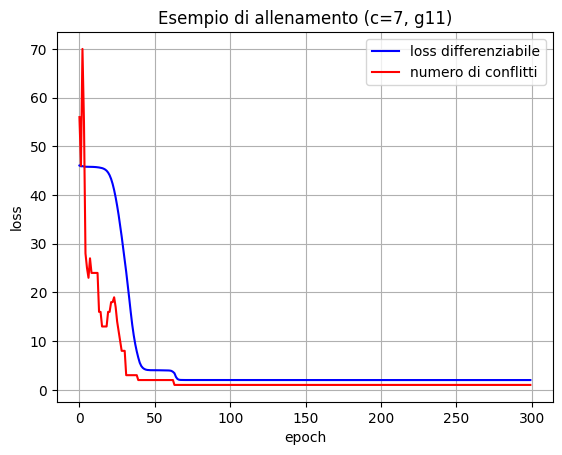
\includegraphics[width = 1 \textwidth]{g11Allenamento}
    \caption{Allenamento di una istanza con g11.}
  \end{subfigure}
  \hfill
  \begin{subfigure}{0.45 \textwidth}
    \centering
    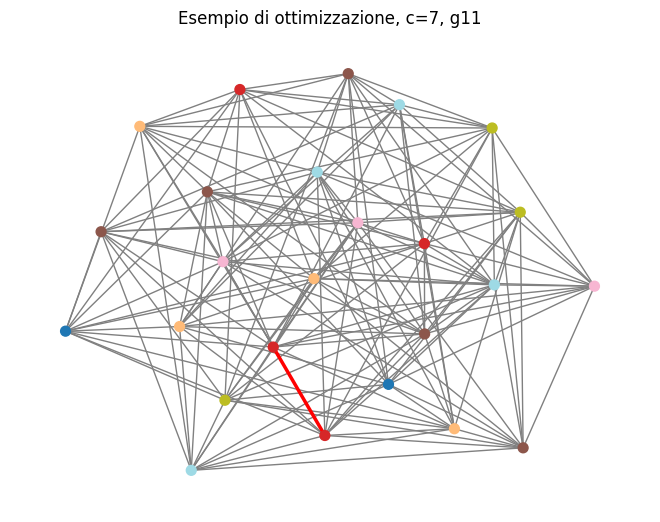
\includegraphics[width = 1 \textwidth]{g11Color}
    \caption{Colorazione trovata dalla GNN, in rosso sono evidenziati i conflitti.}
  \end{subfigure}
    \caption{Allenamento della rete sul grafo g11 e colorazione trovata.}
  \label{fig:g11Soluzione}
\end{figure}

 \begin{figure}[htb!]
  \centering
  \begin{subfigure}{0.45 \textwidth}
    \centering
    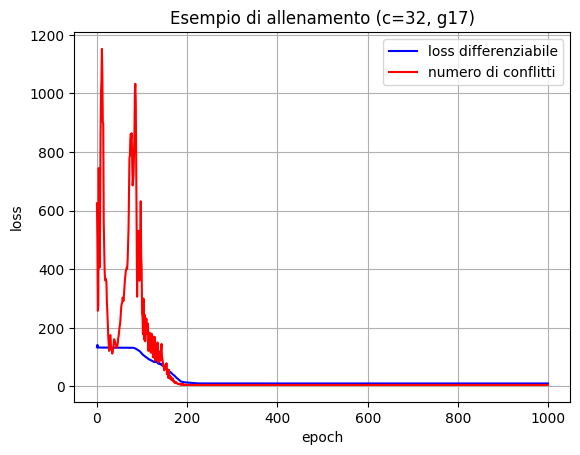
\includegraphics[width = 1 \textwidth]{g17Allenamento}
    \caption{Allenamento di una istanza con g17.}
  \end{subfigure}
  \hfill
  \begin{subfigure}{0.45 \textwidth}
    \centering
    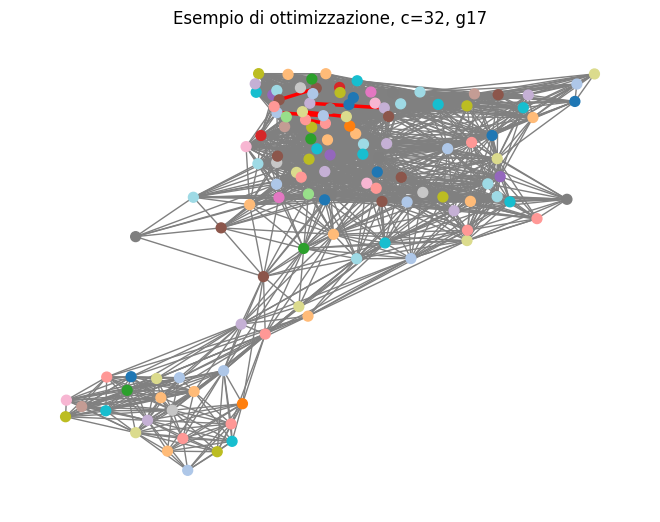
\includegraphics[width = 1 \textwidth]{g17Color}
    \caption{Colorazione trovata dalla GNN, in rosso sono evidenziati i conflitti.}
  \end{subfigure}
    \caption{Allenamento della rete sul grafo g17 e colorazione trovata.}
  \label{fig:g17Soluzione}
\end{figure}
Come riferimento, si è calcolata una colorazione con l'algoritmo greedy \texttt{greedy\_color}
di NetworkX con strategia \textit{largest\_first} (i nodi sono elaborati in ordine di grado
decrescente). Questa euristica classica non garantisce la colorazione ottima, ma fornisce un
limite superiore immediato per $\chi(G)$ e permette di valutare se la GNN migliora rispetto
all'approccio combinatorio semplice.
\section{Risultati}

\subsection*{Grafo \texttt{g11}}

Il grafo \texttt{g11} ha $|V| = 25$ nodi e $|E| = 160$ archi non orientati (rapporto
archi/nodi $\approx 6.4$). La baseline greedy produce una colorazione con $c = 7$ colori.

I risultati dell'ensemble con 50 esecuzioni indipendenti per ciascun valore di $c$, con
400 epoche e $\lambda = 0.05$, sono riportati nella Tabella~\ref{tab:g11}.

\begin{table}[h]
\centering
\caption{Risultati ensemble su \texttt{g11} (50 esecuzioni, 400 epoche, $\lambda = 0.05$, $h = 128$).}
\label{tab:g11}
\begin{tabular}{cccc}
\toprule
$c$ (colori) & Media conflitti & Dev.\ std conflitti & Colorazioni valide \\
\midrule
2 & 123.44 & 1.39 & 0/50 \\
3 & 61.04  & 1.80 & 0/50 \\
4 & 30.80  & 3.67 & 0/50 \\
5 & 12.36  & 5.62 & \textbf{5/50} \\
6 &  4.36  & 3.01 & 11/50 \\
7 &  1.44  & 1.92 & 28/50 \\
8 &  0.36  & 0.77 & 41/50 \\
\bottomrule
\end{tabular}
\end{table}

Il numero medio di conflitti diminuisce monotonicamente all'aumentare di $c$, come atteso. Il comportamento della
deviazione standard è particolarmente informativo: il valore elevato per $c = 5$ (5.62)
indica che in quella regione critica il risultato è molto sensibile all'inizializzazione
casuale, con alcune esecuzioni che trovano la colorazione ottima e altre che restano
intrappolate in minimi locali con molti conflitti.

Con $c = 5$, 5 esecuzioni su 50 (10\%) hanno prodotto una colorazione con zero conflitti.
Poiché è stata concretamente trovata una colorazione valida con 5 colori, si può affermare
con certezza che $\chi(\texttt{g11}) \leq 5$. Il risultato migliora notevolmente la
baseline greedy, che usava 7 colori.

Con $c = 4$, nessuna delle 50 esecuzioni ha trovato una colorazione valida e la media dei
conflitti (30.8) è molto alta. Questo suggerisce con forza che $\chi(\texttt{g11}) > 4$,
pur non costituendo una prova matematica (il metodo GNN potrebbe semplicemente fallire
l'ottimizzazione anche quando la soluzione esiste). La stima più probabile è dunque
$\chi(\texttt{g11}) = 5$.
In Figura \ref{fig:g11Risultati} si riportano i grafici con quanto mostrato nella Tabella.

 \begin{figure}[htb!]
  \centering
  \begin{subfigure}{0.45 \textwidth}
    \centering
    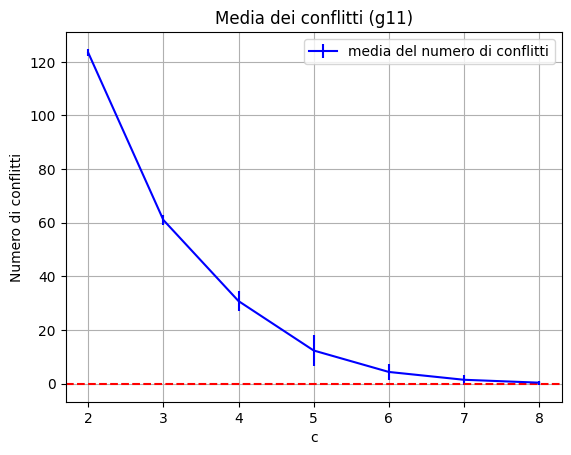
\includegraphics[width = 1 \textwidth]{g11Conflitti}
    \caption{Andamento dei conflitti al variare del numero di colori, si riportano le deviazioni standard misurate.}
  \end{subfigure}
  \hfill
  \begin{subfigure}{0.45 \textwidth}
    \centering
    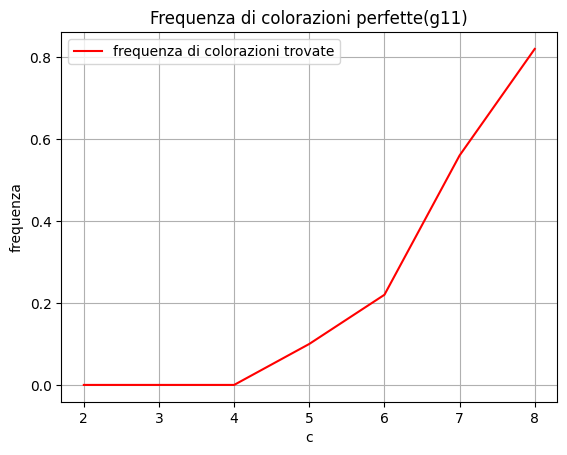
\includegraphics[width = 1 \textwidth]{g11Frequenze}
    \caption{Frequenza del numero di soluzioni trovate al variare del numero di colori, si noti come a partire da $c=5$ ci siano già delle soluzioni.}
  \end{subfigure}
    \caption{Risultati della rete neurale su più realizzazioni.}
  \label{fig:g11Risultati}
\end{figure}

\subsection*{Grafo \texttt{g17}}

Il grafo \texttt{g17} ha $|V| = 128$ nodi e $|E| = 2113$ archi non orientati (rapporto
archi/nodi $\approx 16.5$). La baseline greedy produce una colorazione con $c = 32$
colori. La scansione è stata effettuata a partire da $c = 30$ (leggermente al di sotto
della baseline) fino a $c = 37$, con 50 esecuzioni e 500 epoche ciascuna.

\begin{table}[h]
\centering
\caption{Risultati ensemble su \texttt{g17} (50 esecuzioni, 500 epoche, $\lambda = 0.05$--$0.1$, $h = 128$).}
\label{tab:g17}
\begin{tabular}{cccc}
\toprule
$c$ (colori) & Media conflitti & Dev.\ std conflitti & Colorazioni valide \\
\midrule
30 & 7.14 & 1.18 & 0/50 \\
31 & 6.36 & 1.15 & 0/50 \\
32 & 5.2 & 0.97 & 0/50 \\
33 & 4.66 & 0.88 & 0/50 \\
34 & 3.82 & 0.87 & 0/50 \\
35 & 2.74 & 0.77 & \textbf{1/50} \\
36 & 2.14 & 0.90 & 3/50 \\
37 & 1.76 & 0.88 & 6/50 \\
\bottomrule
\end{tabular}
\end{table}

Per \texttt{g17}, il primo valore di $c$ per cui il metodo ha trovato colorazioni valide
è $c = 35$ (1 esecuzioni su 50, ossia il 2\%). Con $c = 37$ si ottengono 5 colorazioni
valide su 50 (10\%). Si conclude quindi che $\chi(\texttt{g17}) \leq 35$.

Il tasso di successo è decisamente inferiore rispetto a \texttt{g11} a parità di distanza
dalla soglia critica, il che riflette la maggiore difficoltà combinatoria del grafo: con
2113 archi su 128 nodi, i vincoli di colorazione sono molto più fitti e i minimi locali
della loss più numerosi.

Per valori $c \leq 34$, nessuna delle 50 esecuzioni ha prodotto una colorazione valida.
La media dei conflitti decresce lentamente ma non raggiunge lo zero, indicando che queste
configurazioni sono probabilmente al di sotto del numero cromatico. 
\section{Discussione}

\subsection*{Il metodo converge sempre?}

Il metodo converge nel senso che la funzione di loss differenziabile
$\mathcal{L}_{\mathrm{tot}}$ tende a diminuire nel corso del training in quasi tutte le
esecuzioni. Tuttavia, la convergenza della loss \emph{non} implica la convergenza a una
colorazione valida. Il problema è non convesso e la superficie di perdita presenta numerosi
minimi locali, molti dei quali corrispondono a colorazioni discrete con conflitti residui.
In pratica, la rete converge quasi sempre a qualcosa, ma ciò che trova non è necessariamente
la soluzione ottima. Per valori di $c$ molto superiori al numero cromatico la probabilità
di trovare una colorazione valida è alta (82\% per \texttt{g11} con $c = 8$), mentre per
valori vicini a $\chi(G)$ la convergenza è instabile e il risultato dipende fortemente
dall'inizializzazione.

\subsection*{Quanto dipende dall'inizializzazione casuale?}

La dipendenza dall'inizializzazione casuale è molto marcata nella regione critica, cioè
per valori di $c$ prossimi a $\chi(G)$. Per \texttt{g11} con $c = 5$, solo il 10\% delle
esecuzioni trova la colorazione valida, con una deviazione standard dei conflitti di 5.62,
quasi la metà della media stessa (12.36). Per \texttt{g17} con $c = 36$, la frequenza di
successo è solo del 6\%. Questo comportamento è atteso: il problema è NP-difficile,
l'inizializzazione determina il bacino di attrazione in cui cade l'ottimizzatore, e la
superficie di energia è molto corrugata vicino alla soglia critica. Man mano che $c$
aumenta, la dipendenza dall'inizializzazione si riduce (per $c = 8$ su \texttt{g11} il
tasso di successo sale all'82\%), poiché con più colori disponibili i vincoli si allentano
e i minimi locali validi diventano più densi e più facilmente raggiungibili.

\subsection*{Quali valori di $c$ risultano sufficienti?}

Per \texttt{g11}, il metodo trova colorazioni valide a partire da $c = 5$ (con bassa
frequenza) e in modo più affidabile da $c = 7$ in su. La stima del numero cromatico è
$\chi(\texttt{g11}) = 5$, significativamente inferiore alla baseline greedy di 7: il
metodo GNN è quindi in grado di migliorare rispetto all'euristica classica.

Per \texttt{g17}, il primo $c$ con colorazioni valide è 36, superiore alla baseline greedy
di 32. Questo risultato apparentemente controintuitivo riflette la difficoltà
dell'ottimizzazione su un grafo grande e denso: l'algoritmo greedy, essendo deterministico
e costruttivo, spesso trova soluzioni buone più facilmente di un metodo stocastico non
convesso. La stima del numero cromatico per \texttt{g17} è $\chi(\texttt{g17}) \leq 36$,
ma il valore reale potrebbe essere inferiore (fino a 30 o meno): lo strumento GNN non è
riuscito a trovarlo nel regime testato.

\subsection*{Ci sono casi in cui la loss diminuisce ma rimangono conflitti?}

Sì, questo fenomeno è osservato frequentemente, in particolare per valori di $c$ bassi
rispetto al numero cromatico. L'energia di Potts $\mathcal{L}_{\mathrm{Potts}}$ è una
misura di sovrapposizione \emph{continua}: la rete la riduce avvicinando le distribuzioni
di colore di nodi adiacenti su colori diversi, ma la sovrapposizione può essere ridotta
anche con distribuzioni ``morbide'' (softmax non concentrate su un singolo colore) che non
producono ancora una colorazione discreta valida. Dopo la discretizzazione via argmax, le
piccole ambiguità nelle distribuzioni possono generare conflitti che la loss continua non
cattura. In alcuni casi, la loss continua raggiunge un plateau basso mentre il numero di
conflitti discreti rimane costante o addirittura varia in modo non monotono. Questo mette
in evidenza il \textbf{gap tra ottimizzazione continua e problema discreto}, che
rappresenta una limitazione strutturale dell'approccio.

\subsection*{Quali sono i limiti del metodo?}
\begin{itemize}
    \item \textbf{Assenza di garanzie di ottimalità}: essendo la loss non convessa, il
    metodo non garantisce di trovare la colorazione ottima né di certificare che un dato
    $c$ sia inferiore al numero cromatico.
    \item \textbf{Scalabilità}: il metodo richiede di addestrare una rete separata per
    ogni grafo e per ogni valore di $c$, con decine di esecuzioni indipendenti. Questo è
    computazionalmente costoso per grafi molto grandi.
    \item \textbf{Gap discreto-continuo}: la funzione di loss continua e il numero di
    conflitti discreti sono metriche diverse che possono divergere, rendendo difficile
    usare la loss come guida affidabile verso una colorazione valida.
    \item \textbf{Sensibilità agli iperparametri}: le prestazioni dipendono dalla scelta di
    learning rate, peso entropico, numero di epoche e dimensione nascosta. Una
    calibrazione empirica è necessaria per ogni grafo.
    \item \textbf{Stima solo upper bound}: il metodo può dimostrare che $\chi(G) \leq c$
    (trovando una colorazione valida), ma non può dimostrare che $\chi(G) > c$ (un
    fallimento nell'ottimizzazione non esclude l'esistenza della soluzione).
    \item \textbf{Termine entropico}: il termine $\lambda H$ implementato, nella formulazione
    adottata ($H = \frac{1}{|V|}\sum_{ik} p_{ik}\log p_{ik}$), incoraggia distribuzioni
    \emph{uniformi} piuttosto che concentrate. Sebbene questo funzioni come meccanismo di
    esplorazione (tipo annealing), la formulazione della descrizione del progetto prevedeva
    invece di penalizzare l'entropia per favorire assegnazioni nette: invertendo il segno
    si otterrebbe un effetto diverso e potenzialmente più diretto sulla qualità delle
    soluzioni discrete.
\end{itemize}

\end{document}
